\documentclass{standalone}
\usepackage{tikz}
\usepackage{ctex,siunitx}
\usepackage{tkz-euclide}
\usepackage{amsmath}
\usetikzlibrary{patterns, calc}
\usetikzlibrary {decorations.pathmorphing, decorations.pathreplacing, decorations.shapes,}
\begin{document}
\small
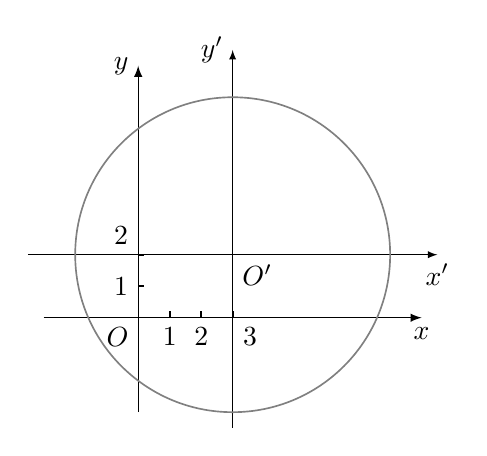
\begin{tikzpicture}[>=latex,scale=0.4]
  \draw[thin,->](-3,0)--(9,0)node[below]{$x$};
  \draw[thin,->](0,-3)--(0,8)node[left]{$y$};
  \draw[very thin,->](-3.5,2)--(9.5,2)node[below]{$x'$};
  \draw[very thin,->](3,-3.5)--(3,8.5)node[left]{$y'$};
  \tkzDefPoints{0/0/O,-2/2/A,3/2/O'}
  \tkzDrawCircle[semithick](O',A)
  \draw[thick](0,1)--++(0.2,0)node[at start,left]{1};
  \draw[thick](0,2)--++(0.2,0)node[at start,above left]{2};
  \foreach \x in {1,2} {\draw[thick](\x,0)--++(0,0.2)node[at start,below]{\x};}
  \draw[thick](3,0)--++(0,0.2)node[at start,below right]{3};
  \tkzLabelPoints[below right](O')
  \tkzLabelPoints[below left](O)
\end{tikzpicture}
\end{document}